\chapter{State of the Art}
\label{chap:\currfilebase}

\section{Measurement}
The process of measurement is the comparison of data from the physical world in the frame of an agreed standard. It is carried out by using an instrument.

This section brings to light some key aspects of measurement instruments and components, used in the frame of this thesis. As a result some sections of \cite{webster2018measurement} are summarized.

\subsection{Measurement and Instrumentation}

Measurement instruments translate signals from the physical world into an agreed upon standard. These standardized signals can be compared, altered and stored.
The original data acquired from the physical signal is usually in analog form. This is then converted to digital before it is passed on. The signal chain of a typical digital measurement instrument is shown in \figref{fig:digital_instrument}.

\cite{webster2018measurement}
\begin{figure}[!htb]
    \centering
    \includestandalone[width=\linewidth]{\imgpath/measurement/digital_instrument/digital_instrument}
    \caption[Digital instrument]{Digital measurement instrument}
    \label{fig:digital_instrument}
\end{figure}

\subsection{Sensors and Transducers}
A device that responds to a changing phenomenon is called sensor. If we need to transfer the energy from one to another, we use a device called transducer. If one compares sensors and transducers based on the energy input and output, one identifies three types:
\begin{itemize}
    \item In \emph{modifiers} a specific energy form is not converted but modified. Hence they use the same form of energy as input and output.
    \item \emph{Self-generators} give out electric signals from non-electric inputs without the need of additional energy.
    \item \emph{Modulators} in contrast give out electric signals from non-electric inputs, but require an additional energy input.
\end{itemize}

As part of this we focus on self-generating piezoelectric sensors, capacitive modulators that convert mechanical deformation in a static electric field into an electric current, as well as strain gauge based modulators.

\subsection{Load Cells}

A force measurement sensor that converts a force into an electrical signal is called \acf{LC}. The basis of force measurement results from the physical behavior of a body under external forces. Depending on the bandwidth and magnitude of the signal, as well as the duration of the signal capture, different methods of force measurement are applied in various designs. The methods in brief are:

\begin{itemize}
    \item Balancing the unknown force against a standard mass through a system of levers
    \item Measuring the acceleration of a known mass
    \item Equalizing it to a magnetic force generated by the interaction of a current-carrying coil and a magnet
    \item Distributing the force on a specific area and then measuring the pressure
    \item Converting the applied force into the deformation of an elastic element
\end{itemize}

Furthermore, these methods yield numerous of designs of measuring equipment. Each of which addressing two main problems. First, the physical and geometrical constrains by the application of the device and second, the means by which the force can be converted into an electrical signal.

\ac{LC}s in \ac{EMA} equipment designs typically use piezoelectric sensors because of their high bandwidth in compact designs and their capability to detect small deflections.

\subsection{Accelerometers}

Accelerometers are sensors that convert acceleration into an electrical signal. In order to measure a physical phenomenon we use seismic masses that act on the sensor structure based on their inertia properties. In strain gauge based accelerometers the structure translates the inertia force into a deformation, where capacitive sensor structures may use deformations or relative motions of separate components in an electric field. In piezoelectric accelerometers the seismic mass deforms a piezoelectric material. \figref{fig:piezo_sensor}
\\[4ex]
\begin{minipage}{\linewidth}
\centering
\begin{minipage}[b]{0.35\textwidth}
    \centering
    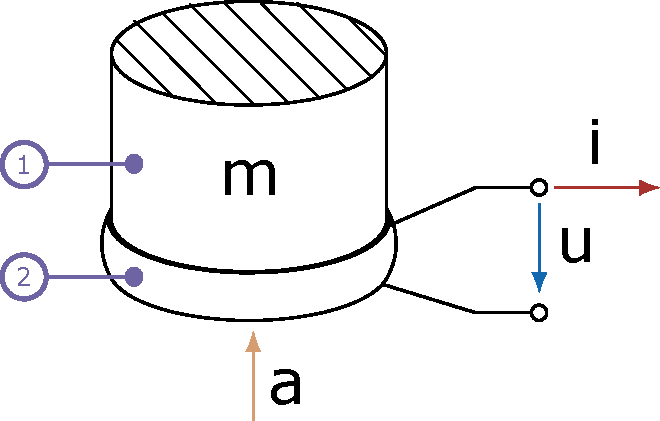
\includegraphics[scale=0.5]{\imgpath/measurement/sensors/piezo_sensor}
    \captionof{figure}[Piezoelectric accelerometer]{Function principle of a piezoelectric accelerometer}
    \label{fig:piezo_sensor}
\end{minipage}
\hspace{4em}
\begin{minipage}[b]{0.3\textwidth}
    \centering
    \footnotesize
    \def\circlabel#1#2{%
        \begin{tikzpicture}[%
            x=1em,y=1ex,
            baseline={([yshift=3] N.south)},
            font={\fontsize{6pt}{6.2pt}\selectfont},
            ]%
            \node[%
                circle, fill=white, draw=#1, line width=1pt,
                inner sep=2pt, minimum size=8pt, align=center,
                ] (N) {#2};
        \end{tikzpicture}
    }
    \begin{tabular}{c@{ :\hskip 0.5em}l}
        \toprule
        \large{a} & Acceleration\\
        \large{m} & Mass\\
        \large{i} & Induced Current\\
        \large{u} & Induced voltage\\
        \large{\circlabel{WesMixL8qual3}{1}} & Seismic mass\\
        \large{\circlabel{WesMixL8qual3}{2}} & Piezoelectric material\\
    \bottomrule
    \end{tabular}
    \normalsize
    \captionof{table}[Legend to piezoelectric accelerometer]{Legend to \figref{fig:piezo_sensor}}
    \label{tab_piezo_sensor}
\end{minipage}
\end{minipage}

In seismic accelerometers the base of the arrangement is motion. When describing the one dimensional case, one can express non-stationary random vibrations acting on the accelerometer as
\begin{align}
    m\dv[2]{z}{t} &= c\dv{z}{t} + kz = mg\cos\pqty{\theta}-m\dv[2]{x_1}{t}
\end{align}
where
\begin{description}[topsep=0ex, noitemsep]
    \item $m$ is the seismic mass
    \item $z=x_2-x_1$ is the relative motion between the mass and the base
    \item $x_1$ is the displacement of the base
    \item $x_2$ is the displacement of the mass
    \item $\theta$ is the angle between sense axis and gravity
\end{description}
The second-order system expressed in Laplace transform thus takes the form
\begin{align}
    G(s) &= \frac{X(s)}{F(s)} \frac{K}{s^2/\omega_n^2 + 2\zeta s/\omega_n + 1}
\end{align}
where
\begin{description}[topsep=0ex, noitemsep]
    \item $s$ is the Laplace operator
    \item $K=1/k$ is the static sensitivity
    \item $\omega_n=\sqrt{k/m}$ is the undamped frequency in \si{\radian\per\second}
    \item $\zeta=c/2\sqrt{km}$ is the damping ratio
\end{description}
It is obvious that the performance of accelerometers depends on their static sensitivity, the natural frequency and the damping ratio. We want the accelerometer to have an linear transfer function in the range of operation. But namely the damping ratio can distort a measurement when operating an accelerometer near its eigenfrequency, see \figref{fig:seismic_accelerometer_edited}.


\begin{figure}[!htb]
    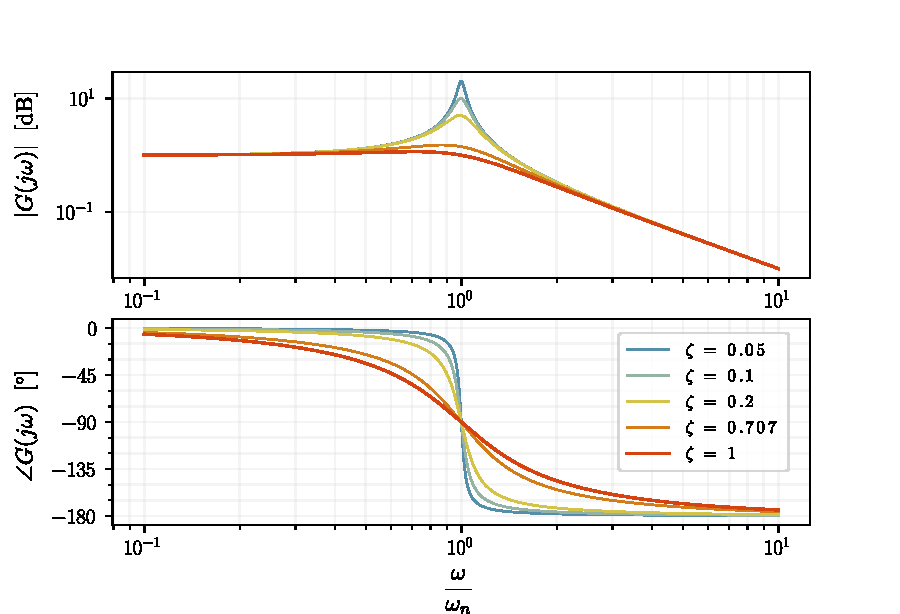
\includegraphics[scale=0.8]{\imgpath/measurement/accel/seismic_accelerometer_edited}
    \caption[Second-Order System Bode plots]{Bode plots of second order system describing the dynamic behavior of seismic accelerometers}
    \label{fig:seismic_accelerometer_edited}
\end{figure}

\subsection{Piezoelectric Sensors}
Some materials develop electric charge proportional to directly applied mechanical stress. The same materials show the converse effect. A proportional strain of the material will occur to an applied electric field.

The first phenomenon has found its application in a variety of self-generating sensors that output electrical signals -- amely in \ac{LC}s and accelerometers, where the piezoelectric charge is converted into a current or voltage signal.

Piezoelectric sensors are designed to exploit the piezoelectric effect of the material in one axis. Additionally, we use amplifier circuits so that the weak current or voltage, induced due to the piezoelectric charge, is elevated to amplitudes that are in the range of operation of standard electronic components. These circuits require additional energy. Commercially available \ac{LC}s therefore require supplied energy -- see \figref{fig:piezo_ampcirc}.

\begin{figure}[!htb]
    \centering
    \subcaptionbox{Piezoelectric sensor connected to a voltage amplifier\label{sfig:piezo_voltage_amp}}{%
        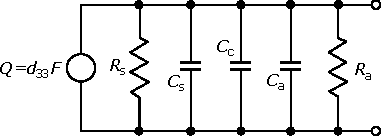
\includegraphics[scale=0.9]{\imgpath/measurement/sensors/piezo_voltage_amp}}
    \hspace{4em}
    \subcaptionbox{Strain gauge in Wheatstone bridge circuit\label{sfig:processing_force_scheme}}{%
        
\includegraphics[scale=0.9]{\imgpath/measurement/sensors/piezo_current_amp}}
    \caption[Piezoelectric sensors in amplifier circuits \cite{webster2018measurement}]{Piezoelectric sensors connected to amplifier circuits \cite{webster2018measurement}}
    \label{fig:piezo_ampcirc}
\end{figure}


\subsection{Strain Gauge Load Cells}

In strain gauge \ac{LC}s the elastic properties of a material probe is exploited.

The probe is loaded in a controlled manner in its elastic region. Deformations are captured by a strain gauge at a suitable location. The probe deformation is directly determined by the force acting on the probe because of Hooke's law.

The strain gauges themselves each use a specific length gauge wire in order to reach a resistance of typically \SI{120}{\ohm}. The wire is bonded between two thin sheets in coiled up form as can be seen in \figref{sfig:strain_gauge}. The sheets act as insulating carrier and can be easily deformed with the intent of passing the load to the wire grid. The gauge is attached to the probe structure by a wax or a resin. The intent is that deformations in transversal direction of the strain gauge act on all coils simultaneously, changing their resistance. By using small sized strain gauges with respect to the probe, the mechanical and thermal properties of the strain gauge become negligible small. As an example, we assume the probe expands. Then a strain gauge on its surface experiences tension. The coils in the grid are therefore stretched and as a result of the generalized Hook's law the coil cross sections decrease. Both the strain in axial direction of the coil and the decreased coil cross sections increase the wire's resistance.

In order to measure deformations one needs to take environmental influences into consideration. It is well known that resistance is susceptible to variations in temperature. Placing the strain gauge in a wheatstone bridge, with resistors, that change their resistance in the same manner as the strain gauge will reduce the influence of temperature significantly -- see \figref{sfig:wheatstone_bridge_single}.

\begin{figure}[!htb]
    \centering
    \subcaptionbox{Strain gauge on structure, with (1) Structure, (2) Metal Pad, (3) Grid and (4) Carrier\label{sfig:wheatstone_bridge_single}}{%
        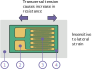
\includegraphics[scale=0.7]{\imgpath/measurement/sensors/strain_gauge}}
    \hspace{4em}
    \subcaptionbox{Strain gauge in Wheatstone bridge circuit\label{sfig:wheatstone_bridge_single}}{%
        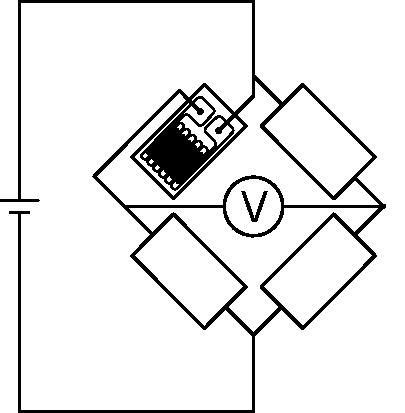
\includegraphics[scale=0.7]{\imgpath/measurement/sensors/wheatstone_bridge_single}}
    \caption[Strain Gauge]{Strain Guage}
\end{figure}

\subsection{Capacitive Accelerometers}

To understand the working principle of capacitive accelerometers, we first consider the displacement sensors.

\subsubsection{Capacitive Displacement Sensors}

The basic sensing element of a displacement sensor typically consists of two parallel electrodes with capacitance C.
\begin{align}
    C &= f(d,A,\varepsilon)
\end{align}

With variable distance, dielectric material or area and with the measurement of the capacitance, we can then deduce the plate displacement in normal and parallel direction to the plates depending on the method used. See \figref{fig:cap_disp} 

In variable displacement sensors, the distance between two capacitive plates is inversely proportional to the capacitance.
\begin{align}
    C(x) &= \frac{\varepsilon A}{x} = \frac{\varepsilon_r\varepsilon_0 A}{x}
\end{align}
where
\begin{description}[topsep=0ex, noitemsep]
    \item $\varepsilon$ is dielectric constant or permittivity
    \item $\varepsilon_r$ is the relative dielectric constant (in air and vacuum $\varepsilon_r\approx 1$)
    \item $\varepsilon_0$ is \SI{8.854188}{\farad\per\meter}, the dielectric constant of vacuum
    \item $x$ is the distance of the plates in \si{\meter}
    \item $A$ is the effective area of the plates in \si{\meter\squared}
\end{description}

In variable area displacement sensors, the capacitance is proportional to the reduction of area due to the movement of the plate.
\begin{align}
   C(x) &= \frac{\varepsilon_r\varepsilon_0\pqty{A-wx}}{d}\label{eqn:var_ar_displace}
\end{align}
where
\begin{description}[topsep=0ex, noitemsep]
    \item $\varepsilon_2$ is the permittivity of the displacing material (e.g. liquid)
    \item $w$ is the width
    \item $wx$ is the reduction in the area due to movement of the plate 
    \item $d$ is the distance of the plates in \si{\meter}
\end{description}

In variable dielectric sensors, the capacitance depends on the ratio of each permittivity in the electric field.
\begin{align}
   C(x) &= \varepsilon_0 w \bqty{\varepsilon_2 l - \pqty{\varepsilon_2-\varepsilon_1}x}\label{eqn:var_diel_displace}\\
\end{align}
where
\begin{description}[topsep=0ex, noitemsep]
    \item $x$ is the displacement normal to the plates direction
    \item $\varepsilon_1$ is the relative permittivity of the dielectric material
    \item $\varepsilon_2$ is the permittivity of the displacing material (e.g. liquid)
\end{description}
Differential capacitive displacement sensors are setup in capacitive arrangements that aim to eliminate nonlinearities. Different variations of these types of sensors exist. For example we can allow the outer plates to move and fix the middle one or we can reverse this setup. But the range is equal to twice the separation in both cases.

\begin{align}
    2\delta C = C_1-C_2 &= \frac{\varepsilon_r\varepsilon_0 lw}{d-\delta d} - \frac{\varepsilon_r\varepsilon_0 lw}{d+\delta d} = \frac{2\varepsilon_r\varepsilon_0 lwd}{d^2+\delta d^2}\\
    C_1+C_2 &= \frac{\varepsilon_r\varepsilon_0 lw}{d-\delta d} + \frac{\varepsilon_r\varepsilon_0 lw}{d+\delta d} = \frac{2\varepsilon_r\varepsilon_0 lwd}{d^2+\delta d^2}\\
\end{align}
Giving approximately
\begin{align}
    \frac{\delta C}{C} = \frac{\delta d}{d}
\end{align}

\begin{figure}[!ht]
    \sbox0{\subcaptionbox{Variable distance displaceement\label{sfig:cap_var_disp}}{%
        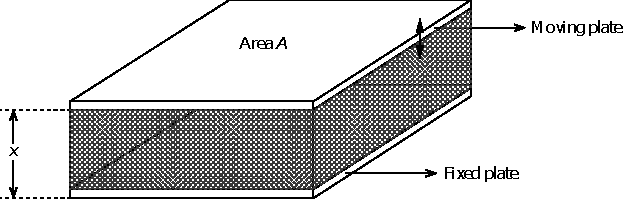
\includegraphics[scale=0.7]{\imgpath/measurement/capac/cap_var_disp}
        }}% a
    \sbox1{\subcaptionbox{Variable area displacement\label{sfig:cap_var_area}}{%
        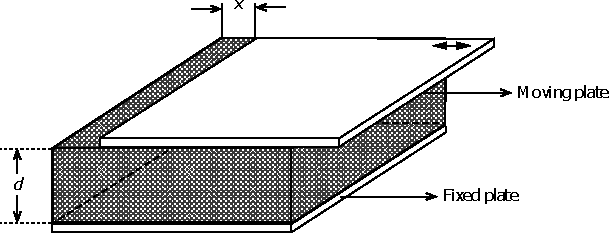
\includegraphics[scale=0.7]{\imgpath/measurement/capac/cap_var_area}
        }}% b
    \sbox2{\subcaptionbox{Variable dielectric displacement\label{sfig:cap_var_diel}}{%
        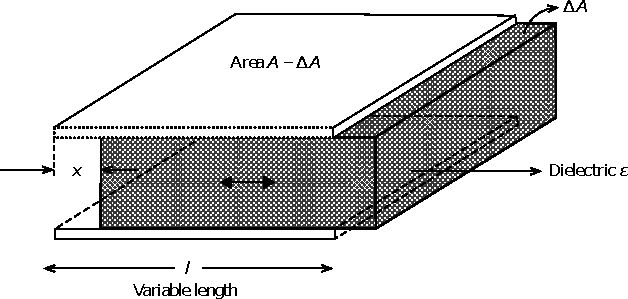
\includegraphics[scale=0.7]{\imgpath/measurement/capac/cap_var_diel}
        }}% c
    \sbox3{\subcaptionbox{Differential capacitive displacement\label{sfig:cap_diff}}{%
        \includegraphics[scale=0.7]{\imgpath/measurement/capac/cap_diff}
        }}% d
    \sbox4{\subcaptionbox{IC smart capacitive displacement \label{sfig:cap_smart}}{%
        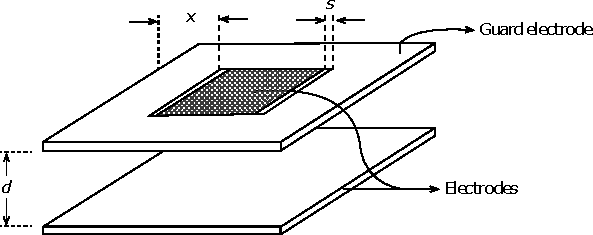
\includegraphics[scale=0.7]{\imgpath/measurement/capac/cap_smart}
        }}% e
    \centering
    {%
        \renewcommand{\arraystretch}{6}%
        \setlength{\tabcolsep}{0em}
        \begin{tabular}{ccc}
            \usebox0 & \usebox1 \\
            \usebox2 & \usebox3 \\
        \end{tabular}\\[4ex]
        \usebox4
    }
    \caption[Capacitive displacement sensors]{Capacitive displacement sensors \cite{webster2018measurement}}
    \label{fig:cap_disp}
\end{figure}

\begin{figure}[!ht]
\sbox0{\subcaptionbox{Vertical stress, longitudinal particle displacement\label{sfig:piezo_beam}}{%
        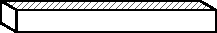
\includegraphics[scale=0.7]{\imgpath/measurement/piezo/piezo_beam}
        }}% a
    \sbox1{\subcaptionbox{Vertical stress, lateral particle displacement\label{sfig:piezo_plate_top}}{%
        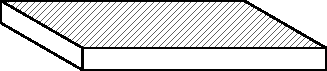
\includegraphics[scale=0.7]{\imgpath/measurement/piezo/piezo_plate_top}
        }}% b
    \sbox2{\subcaptionbox{Vertical stress, lateral particle displacement\label{sfig:piezo_plate_side}}{%
        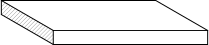
\includegraphics[scale=0.7]{\imgpath/measurement/piezo/piezo_plate_side}
        }}% c
    \sbox3{\subcaptionbox{Lateral stress, lateral particle displacement\label{sfig:piezo_radial_long}}{%
        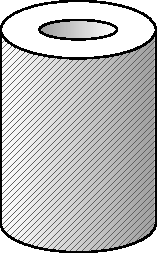
\includegraphics[scale=0.7]{\imgpath/measurement/piezo/piezo_radial_long}
        }}% d
    \sbox4{\subcaptionbox{Radial particle displacement\label{sfig:piezo_radial_flat}}{%
        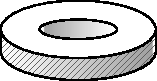
\includegraphics[scale=0.7]{\imgpath/measurement/piezo/piezo_radial_flat}
        }}% e
    \sbox5{\subcaptionbox{Radial particle displacement\label{sfig:piezo_axial_hole_flat}}{%
        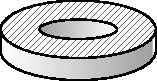
\includegraphics[scale=0.7]{\imgpath/measurement/piezo/piezo_axial_hole_flat}
        }}% f
    \sbox6{\subcaptionbox{Vertical stress, radial particle displacement\label{sfig:piezo_sphere}}{%
        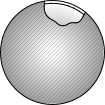
\includegraphics[scale=0.7]{\imgpath/measurement/piezo/piezo_sphere}
        }}% g
    \sbox7{\subcaptionbox{Radial particle displacement\label{sfig:piezo_axial_flat}}{%
        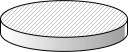
\includegraphics[scale=0.7]{\imgpath/measurement/piezo/piezo_axial_flat}
       }}% h
    \sbox8{\subcaptionbox{Radial particle displacement\label{sfig:piezo_radial_rod}}{%
        
\includegraphics[scale=0.7]{\imgpath/measurement/piezo/piezo_radial_rod}
       }}% i
    \centering
    {%
        \renewcommand{\arraystretch}{4}%
        \setlength{\tabcolsep}{2em}
        \begin{tabular}{ccc}
            \usebox0 & \usebox3 & \usebox6 \\
            \usebox1 & \usebox4 & \usebox7 \\
            \usebox2 & \usebox5 & \usebox8
        \end{tabular}
    }
    \caption[Piezoelectric designs]{Piezoelectric designs, where electrodes are placed on the shaded areas}
    \label{fig:allsix}
\end{figure}

\subsubsection{Capacitive Accelerometers}


\section{Experimental Modal Analysis}

\ac{EMA} is a powerful tool to detect vibration related problems of mechanical structures. We use modes to characterize resonant vibrations of the system
\cite{schwarz1999experimental}


\subsubsection{Vibration}

In every vibration one can observe a combination of two different types of vibrations. The forced and the resonant ones. Forced vibrations in a structure are caused by
\begin{itemize}
    \item Internally generated forces
    \item Unbalances
    \item External loads
    \item Ambient excitations
\end{itemize}
Common examples of vibration sources in \ac{MT} are displayed in \figref{fig:vibration_sources}.

\begin{figure}[!htb]
    \centering
    \subcaptionbox{Axis Motion\label{sfig:ball_screw_simple}}{%
        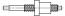
\includegraphics[scale=0.7]{\imgpath/ema/vibration_sources/ball_screw_simple}}
        \hspace{4em}
    \subcaptionbox{Imbalance\label{sfig:imbalance_scheme}}{%
        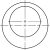
\includegraphics[scale=0.7]{\imgpath/ema/vibration_sources/imbalance_scheme}}
    \hspace{4em}
    \subcaptionbox{Processing Force\label{sfig:processing_force_scheme}}{%
        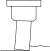
\includegraphics[scale=0.7]{\imgpath/ema/vibration_sources/processing_force_scheme}}
    \\[5ex]
    \begingroup
    \subcaptionbox{Impact Hammer\label{sfig:impulse_hammer_scheme}}[0.5\linewidth]{%
        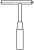
\includegraphics[scale=0.7]{\imgpath/ema/vibration_sources/impulse_hammer_scheme}}
    \endgroup
    \hspace{0em}
    \subcaptionbox{Modal Shaker\label{sfig:modalShaker_scheme}}{%
        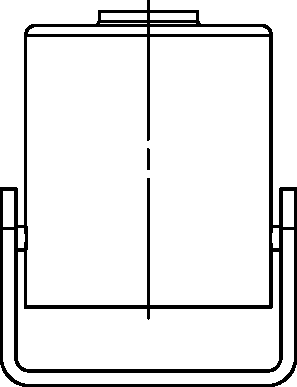
\includegraphics[scale=0.7]{\imgpath/ema/vibration_sources/modalShaker_scheme}}
    \caption[Forced Vibration Sources]{Sources of forced vibration. Note that \subref{sfig:ball_screw_simple}, \subref{sfig:imbalance_scheme} and \subref{sfig:processing_force_scheme} occur during \ac{MT} operation, while \subref{sfig:impulse_hammer_scheme} and \subref{sfig:modalShaker_scheme} are devices that are explicitly used for \ac{EMA} to introduce vibrations into the structure of investigation.}
    \label{fig:vibration_sources}
\end{figure}

Resonant vibration arises when one or more of the natural modes of vibration, inherent properties of the structure under investigation, is excited. Resonant vibration typically amplifies the vibration response to a level that exceeds deflection, stress and strain caused by static loading. 

\subsubsection{Modes}

Modes or resonances are properties that are inherent to a structure. 

\subsection{Frequency Response Measurement}

In a \ac{EMA} one needs to determine the \ac{FRF} from input to output. To achieve this we measure the so called response or output function of the structure under investigation. The measurement instrument for this task uses a signal chain in form of \ref{fig:measurment}.
\begin{itemize}
    \item The sensor on the structure translates the physical value (acceleration, velocity or position) into an electrical voltage or current, the analog signal variable.
    \item The amplifier amplifies the typically low power signal to fit it to the input range of the \ac{ADC}.
    \item The \ac{ADC} samples and quantizes the analog signal. It is then converted into a digital signal, in which the quantity is expressed in form of a binary code.
    \item The discrete time signal is then stored on the computer memory.
\end{itemize}
\cite{fu2001modal}

\begin{figure}[!htb]
    \centering
    \includestandalone[width=\linewidth]{\imgpath/ema/measurment/measurment}
    \caption[Frequency Response Measurement]{\ac{FRF} measurement setup}
    \label{fig:measurment}
\end{figure}

\section{Electronic Components}

This section serves as an introduction to the function of selected electronic components and circuits. It does not give a complete overview of the state of the art. For more background on electronics \todo{cite electronic handbooks} may be consulted.

Electronic components are divided into two main types; passive and active ones. Where active components are allowed to generate, amplify or oscillate an electrical signal, passive components can only absorb, dissipate or store electric energy.

\subsection{Passive Components}

Because of the increase in digital processing, the number of passive components has decreased drastically in modern electronic circuits. This, in addition to the trend of using more complex devices in favour to multiple simple passive components, has led to a great variety of passive components which are designed with emphasis on reliability.

\subsubsection{Wires}

Wires connect several electronic components. Ideally no loss or noise is introduced in wires but inductances occur due to the conductor's shape and material properties as well as electric fields, that are either self induced or present due to ambient conditions.

Depending on the mechanical requirements for the wire, it can either be designed with a solid core or a stranded wire core. A wire consisting of multiple smaller diameter conductors shows better flexibility but reduced current-carrying capacity at the same wire diameter. This is because of the smaller overall conductor cross-section of a stranded wire and, when transmitting high frequency signals, a greater power dissipation due to the more prevalent skin effect. Furthermore the simplicity of solid core wires makes them more resistant to corrosion and more suitable to be used in harsh environments.

Braided or foil shielding wires are usually used to shield other wires from ambient fields. Shaped as a tube they enclose one or multiple wires acting as a Faraday cage.

\subsubsection{Resistors}

Resistors are loads that reduce the current flow and set the voltage levels within a circuit. There are many different types of resistors.

\subsection{Active Components}

\subsection{Integrated Circuits}

\begin{figure}[!htb]
    \centering
    \includestandalone[scale=1]{\imgpath/electronics/ic_flowchart/ic_flowchart}
    \caption[IC packages flowchart]{Flowchart of IC packages}
    \label{fig:ic_flowchart}
\end{figure}

\subsection{Circuits}